\section{Introducción}
Desde el punto de vista observacional, la mayoría de las galaxias están formadas por una región central brillante fácilmente distinguible, que concentra la mayor parte de la masa estelar y la materia más metálica; y por un tenue halo de gran extensión, compuesto de estrellas dispersas y más antiguas \nota{incluir cita}. En ausencia de influencias externas, las galaxias elípticas, las más evolucionadas \nota{?} y estables, presentan un perfil suave y homogéneo en el que la intensidad de la luz decae progresivamente con la distancia al centro \nota{cita?} \nota{imagen de una galaxia elíptica prototípica}. \par

Sin embargo, la interacción con otras galaxias puede perturbar ese equilibrio e introducir inhomogeneidades en el halo estelar. La naturaleza de las inhomogeneidades depende del tipo de interacción, las circunstancias en las que esta se produjo y el tiempo transcurrido desde que sucedió. Por este motivo, el estudio del halo estelar de las galaxias nos aporta información fundamental para determinar los sucesos que influyeron en su desarrollo. Dado que el modelo cosmológico estándar otorga una gran importancia a los eventos de colisión y fusión de galaxias para explicar la evolución del universo \autocite{bullockTracingGalaxyFormation2005,popFormationIncidenceShell2018}, podemos afirmar que el análisis de las estructuras de bajo brillo superficial en las galaxias elípticas tiene un gran interés físico. \par 

Como hemos mencionado, existen varios tipos de estructuras que podemos encontrar en el halo estelar, que representamos de manera no exhaustiva en la figura \ref{tidalfeats}. Un ejemplo son las corrientes de marea (\textit{tidal streams}), que trazan \enquote{lazos} alrededor de las galaxias \autocite{newbergIntroductionTidalStreams2016,martinez-delgadoDISCOVERYGIANTStelLAR2009}, y que parecen estar formadas por estrellas arrancadas de galaxias satélite que orbitaban con un momento angular relativamente alto \autocite{popFormationIncidenceShell2018}. Otro tipo de estructuras son los penachos (\textit{plumes}) \nota{desarrollar}. Las \enquote{shells} \nota{traducción?}, por su parte, son regiones curvas y regulares, frecuentemente presentes en torno al eje mayor de la galaxia, en las que se observa un exceso de brillo superficial en comparación con sus alrededores, y dispuestas de manera que forman \enquote{capas} bien definidas. \nota{Referencia donde haya una lista más exhaustiva?}\par \label{estructuras}

\begin{figure}[h]
\centering
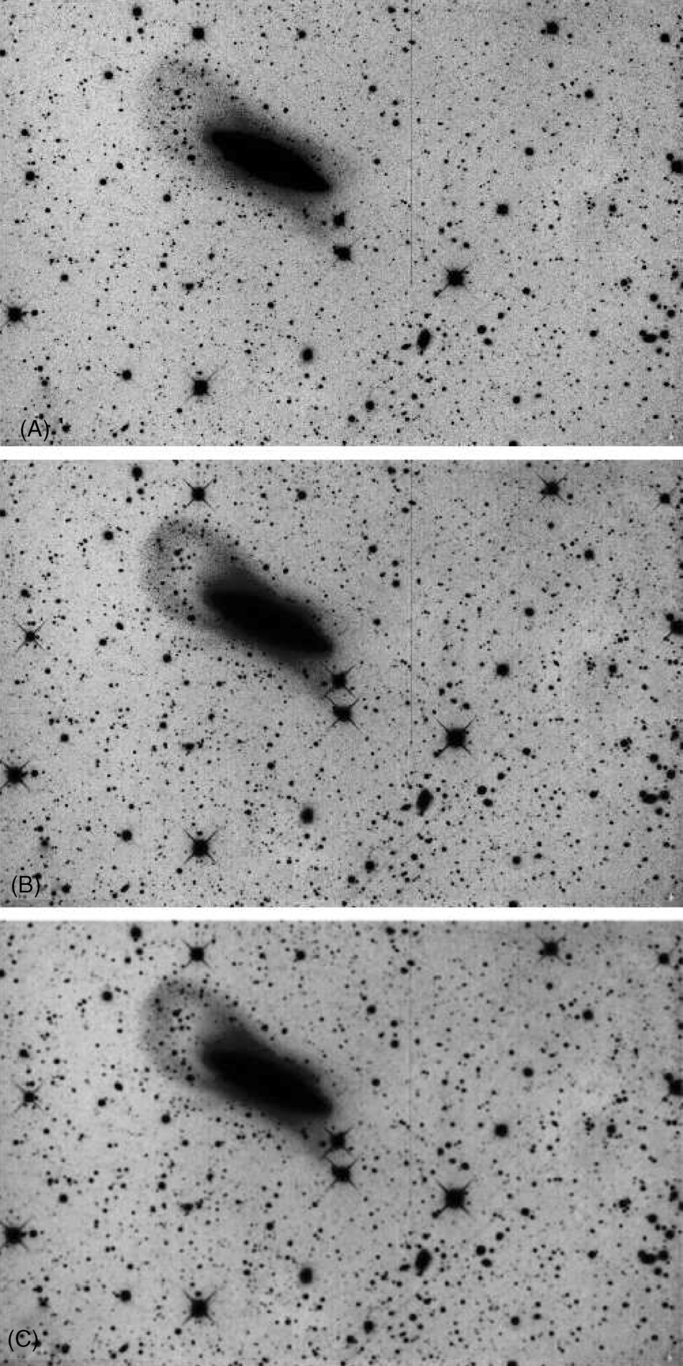
\includegraphics[trim={10 70 20 60}, clip, width=0.4\textwidth]{tidalstream.jpg}
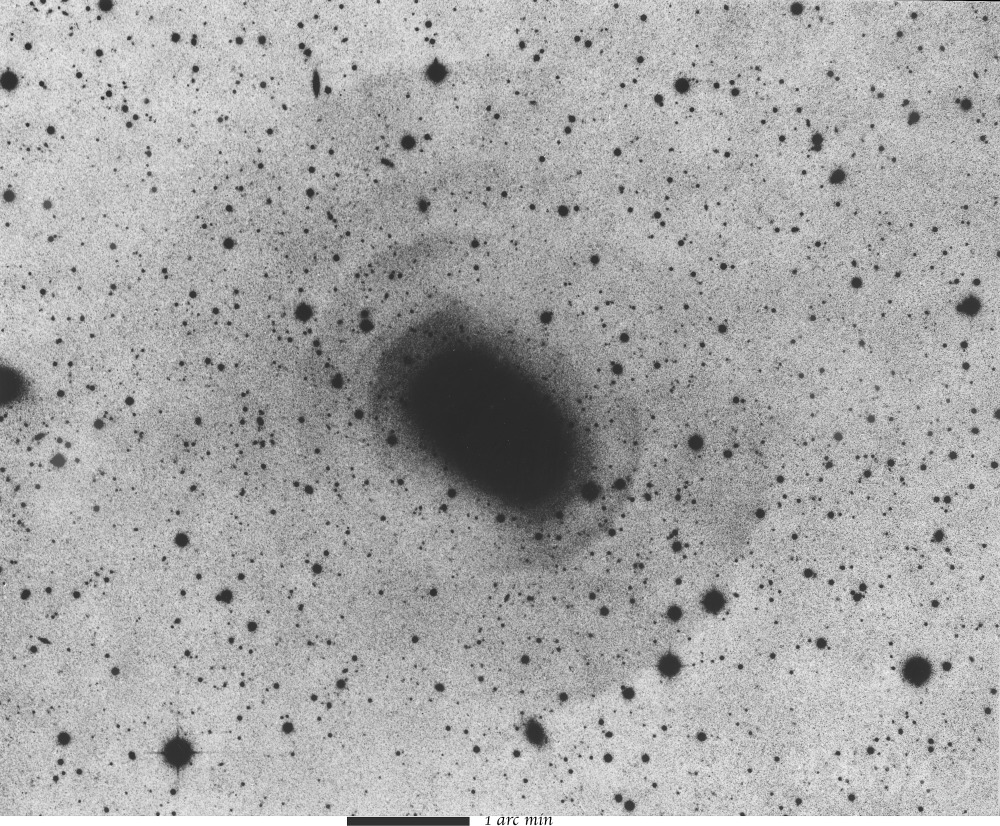
\includegraphics[trim={0 10 0 0}, clip, width=0.4\textwidth]{shellsmalin.jpg}			
\caption{\nota{escribir pie de figura} \autocite{martinez-delgadoDISCOVERYGIANTStelLAR2009} \autocite{malinInnerShellsElliptical,malinGiantShellsNormal1980} \label{tidalfeats}}
\end{figure}
\noindent

Este trabajo se centrará en el estudio de las shells del cúmulo relajado de galaxias \cluster, identificado en \autocite{jimenez-tejaFirstJointMUSE2024} como un lugar de alto interés para el análisis de estas estructuras. A lo largo de esta introducción, detallaremos los últimos avances en los modelos de formación de shells \nota{explicar lo que se va a hacer}

\subsection{Formación de shells. La simulación Illustris.}
Las primeras observaciones de galaxias con shells se publicaron en el Atlas de galaxias peculiares de 1966 \autocite{arpAtlasPeculiarGalaxies1966}. En aquel momento, el bajo brillo superficial de estas estructuras impedía un análisis sistemático de sus propiedades. Años más tarde, la aplicación de técnicas de amplificación fotográfica en \autocite{malinCatalogEllipticalGalaxies1983} permitió la identificación de 137 galaxias elípticas con shells. Solamente 5 de ellas se encontraban en cúmulos, y la mayoría estaban aisladas o en grupos de pocas galaxias. De hecho, de entre las galaxias elípticas aisladas incluidas en el estudio, las galaxias con shells representaban un 17\%, cifra muy superior a la alcanzada para los grupos más numerosos y los cúmulos. Estos resultados ya sugerían una de las condiciones que favorecen la estabilidad de las shells: un ambiente frío y estable que no facilite la difusión de las estrellas en el halo. \nota{encajar con lo de después, mencionar que es tb posiblemente un efecto observacional} \par

\nota{desarrollar con algunas de las observaciones de shells desde entonces, tampoco mucho, y los tipos I II y III}

Debido a que no podemos observar directamente la evolución del proceso de formación de una shell ni de ninguna otra estructura, el uso de simulaciones es imprescindible para poder elaborar modelos y sugerir características en las que centrarse en los análisis de galaxias reales. La más destacada de estas simulaciones hasta la fecha es Illustris. \par

El proyecto Illustris utilizó el modelo cosmológico estándar \(\Lambda\)CDM para elaborar una simulación hidrodinámica-gravitatoria a gran escala del universo centrada en la formación y evolución de las galaxias, comenzando en \(z = 137\) (aproximadamente 12 millones de años tras el Big Bang) y concluyendo en la actualidad \autocite{vogelsbergerPropertiesGalaxiesReproduced2014,vogelsbergerIntroducingIllustrisProject2014}. Incorporaron modelos astrofísicos para la formación y evolución de estrellas, agujeros negros supermasivos, y otros efectos como los vientos galácticos o las emisiones radiativas de los núcleos activos galácticos (AGN). La resolución obtenida es tan alta que es posible analizar en detalle características internas de las galaxias como, por ejemplo, su composición química. En \(z=0\) la simulación es capaz de producir una muestra de aproximadamente 40000 galaxias y 600 millones de \enquote{partículas estelares}, obteniendo una población de objetos astrofísicos muy variada y que reproduce razonablemente bien las observaciones. \par

En \autocite{popFormationIncidenceShell2018} se aprovecharon estos resultados para analizar en profundidad las formación y evolución de las shells en las galaxias más masivas de Illustris. A lo largo del resto de esta sección resumiremos los hallazgos más destacados de este estudio. \par

Se analizaron las 220 galaxias más masivas de la simulación en \(z = 0\), que cuentan con masas estelares \(M_{stars} \gtrsim 10^{11}_{\odot}\) (como comparación, la Vía Láctea tiene una masa estelar estimada del orden de \(10^{10} \, M_{\odot}\), aunque existen discrepancias sobre el valor exacto \autocite{lianErratumMilkyWay2026, bovyDIRECTDYNAMICALMEASUREMENT2013}). La identificación de las shells se hizo de manera visual, como se haría con la observación de una galaxia real. Sin embargo, la simulación permite seguir a cada partícula estelar de manera independiente para diferentes \(z\), asociando con ella tres parámetros: el tiempo de formación \(t_{form}\) de la estrella; el tiempo de acreción \(t_{acc}\), que señala el momento en que la partícula estelar entra en el radio del virial de la galaxia\footnote{El radio del virial de la galaxia se define como el radio que encierra una esfera con una densidad media 200 veces superior a la densidad crítica del universo. \label{virial}}; y el tiempo de extracción \(t_{strip}\) \nota{traducción?}, el momento en el que la estrella queda atrapada en el campo gravitatorio de la galaxia a estudiar. \par

Con estos parámetros se pueden definir dos tipos de estrellas: las estrellas \textit{in situ} se formaron ya en la galaxia, de manera que \(t_{form} = t_{acc} = t_{strip}\); mientras que las \textit{ex situ} proceden de galaxias externas, y por lo tanto \(t_{form} > t_{acc} > t_{strip}\) \nota{traducción de lookback?}. Inmediatamente podemos ver en la figura \ref{shellspop} que las responsables de formar las shells son las estrellas \textit{ex situ}. Además, en esta figura no solo podemos distinguir las shells en el espacio de configuración \((x, y)\), sino también en el espacio de fases \((r, v_{r})\), siendo \(r\) la distancia galactocéntrica de cada estrella y \(v_{r}\) su velocidad radial.

\begin{figure}[h]
\centering
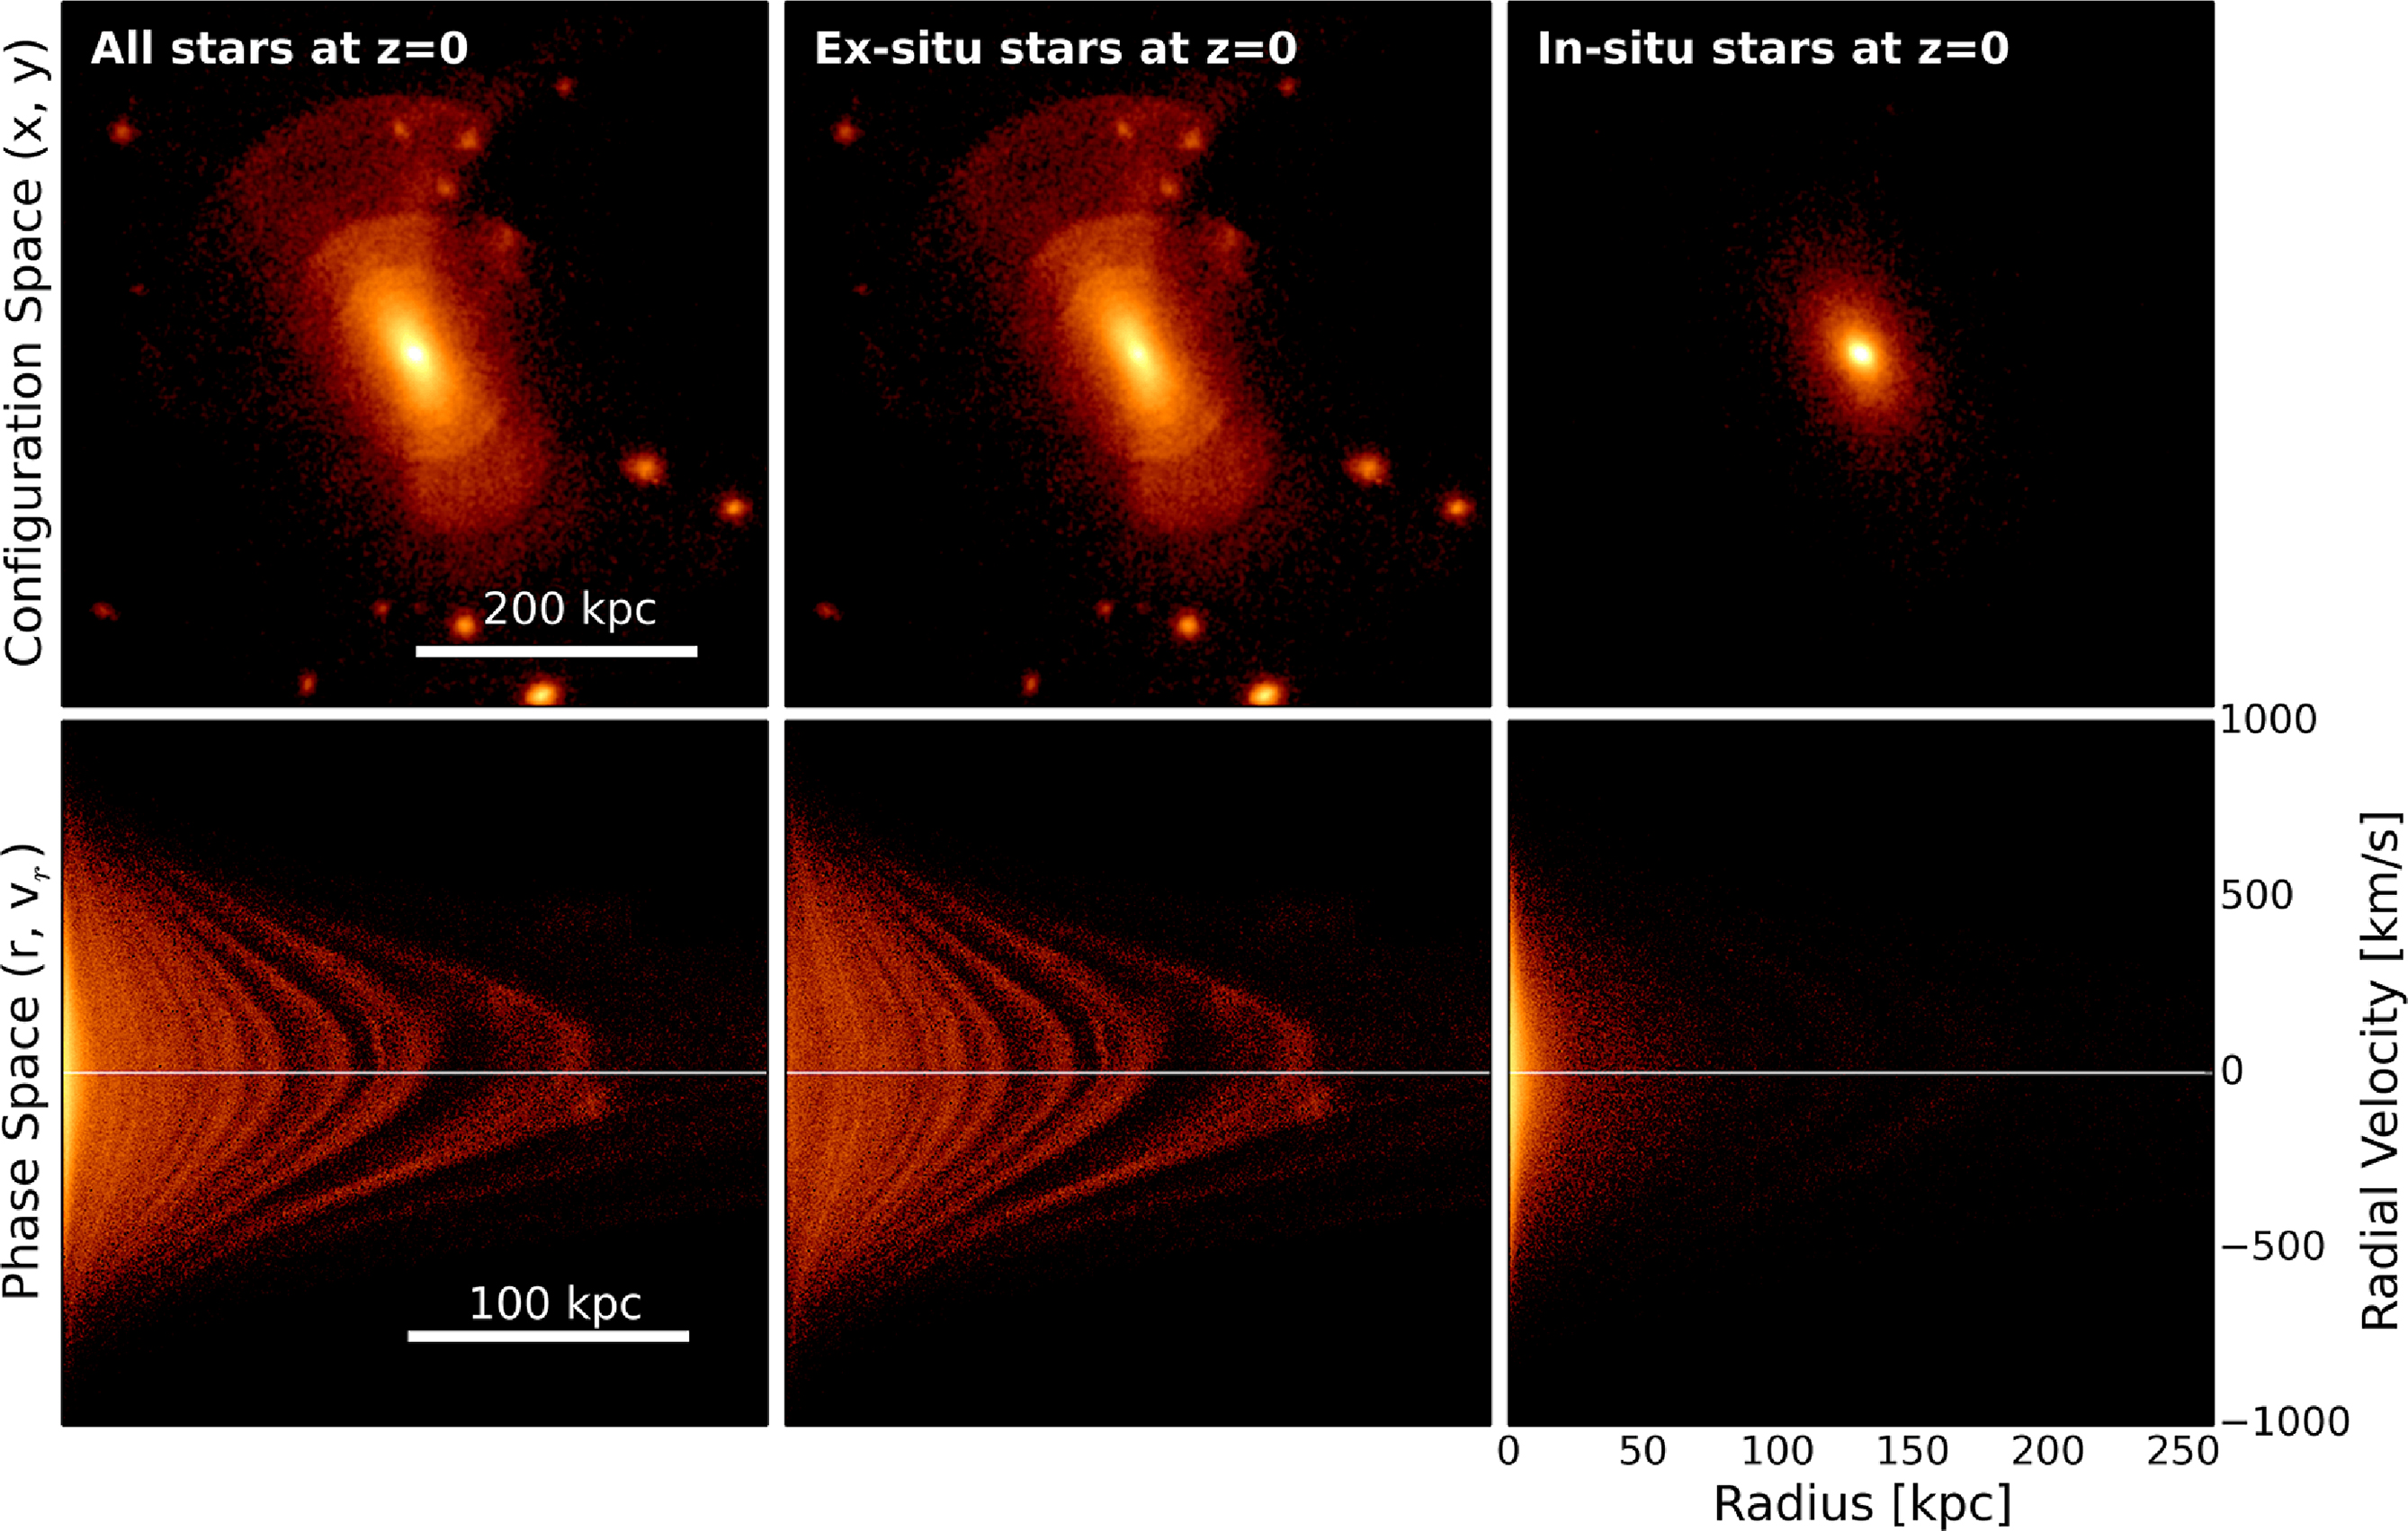
\includegraphics[trim={0 0 0 0}, clip, width=0.9\textwidth]{shellspop1.jpeg}			
\caption{En esta galaxia de Illustris podemos observar varias shells bien definidas, tanto en el espacio de configuración \((x,y)\) como en el de fases \((r, v_{r})\). Distinguiendo entre estrellas \textit{in situ} y \textit{ex situ}, vemos que las primeras se concentran cerca del centro y están bien mezcladas, mientras que las segundas se extienden a distancias grandes y se concentran cerca del apoastro de órbitas concretas. Imagen de \autocite{popFormationIncidenceShell2018} (figura 2). \label{shellspop}}
\end{figure}
\noindent



En total, se identificaron 39 galaxias con shells (un 18\%), cifra comparable a la observada en \autocite{malinCatalogEllipticalGalaxies1983}. Sin embargo, analizando detenidamente la distribución de masa (representada en la figura \ref{shellmass}) se observa que esta proporción es mayor cuanto mayor es la masa que se considera, lo que justifica el haberse centrado únicamente en las galaxias más grandes. Trataremos la justificación física de esta cuestión más adelante. \par


\begin{figure}[h]
\centering
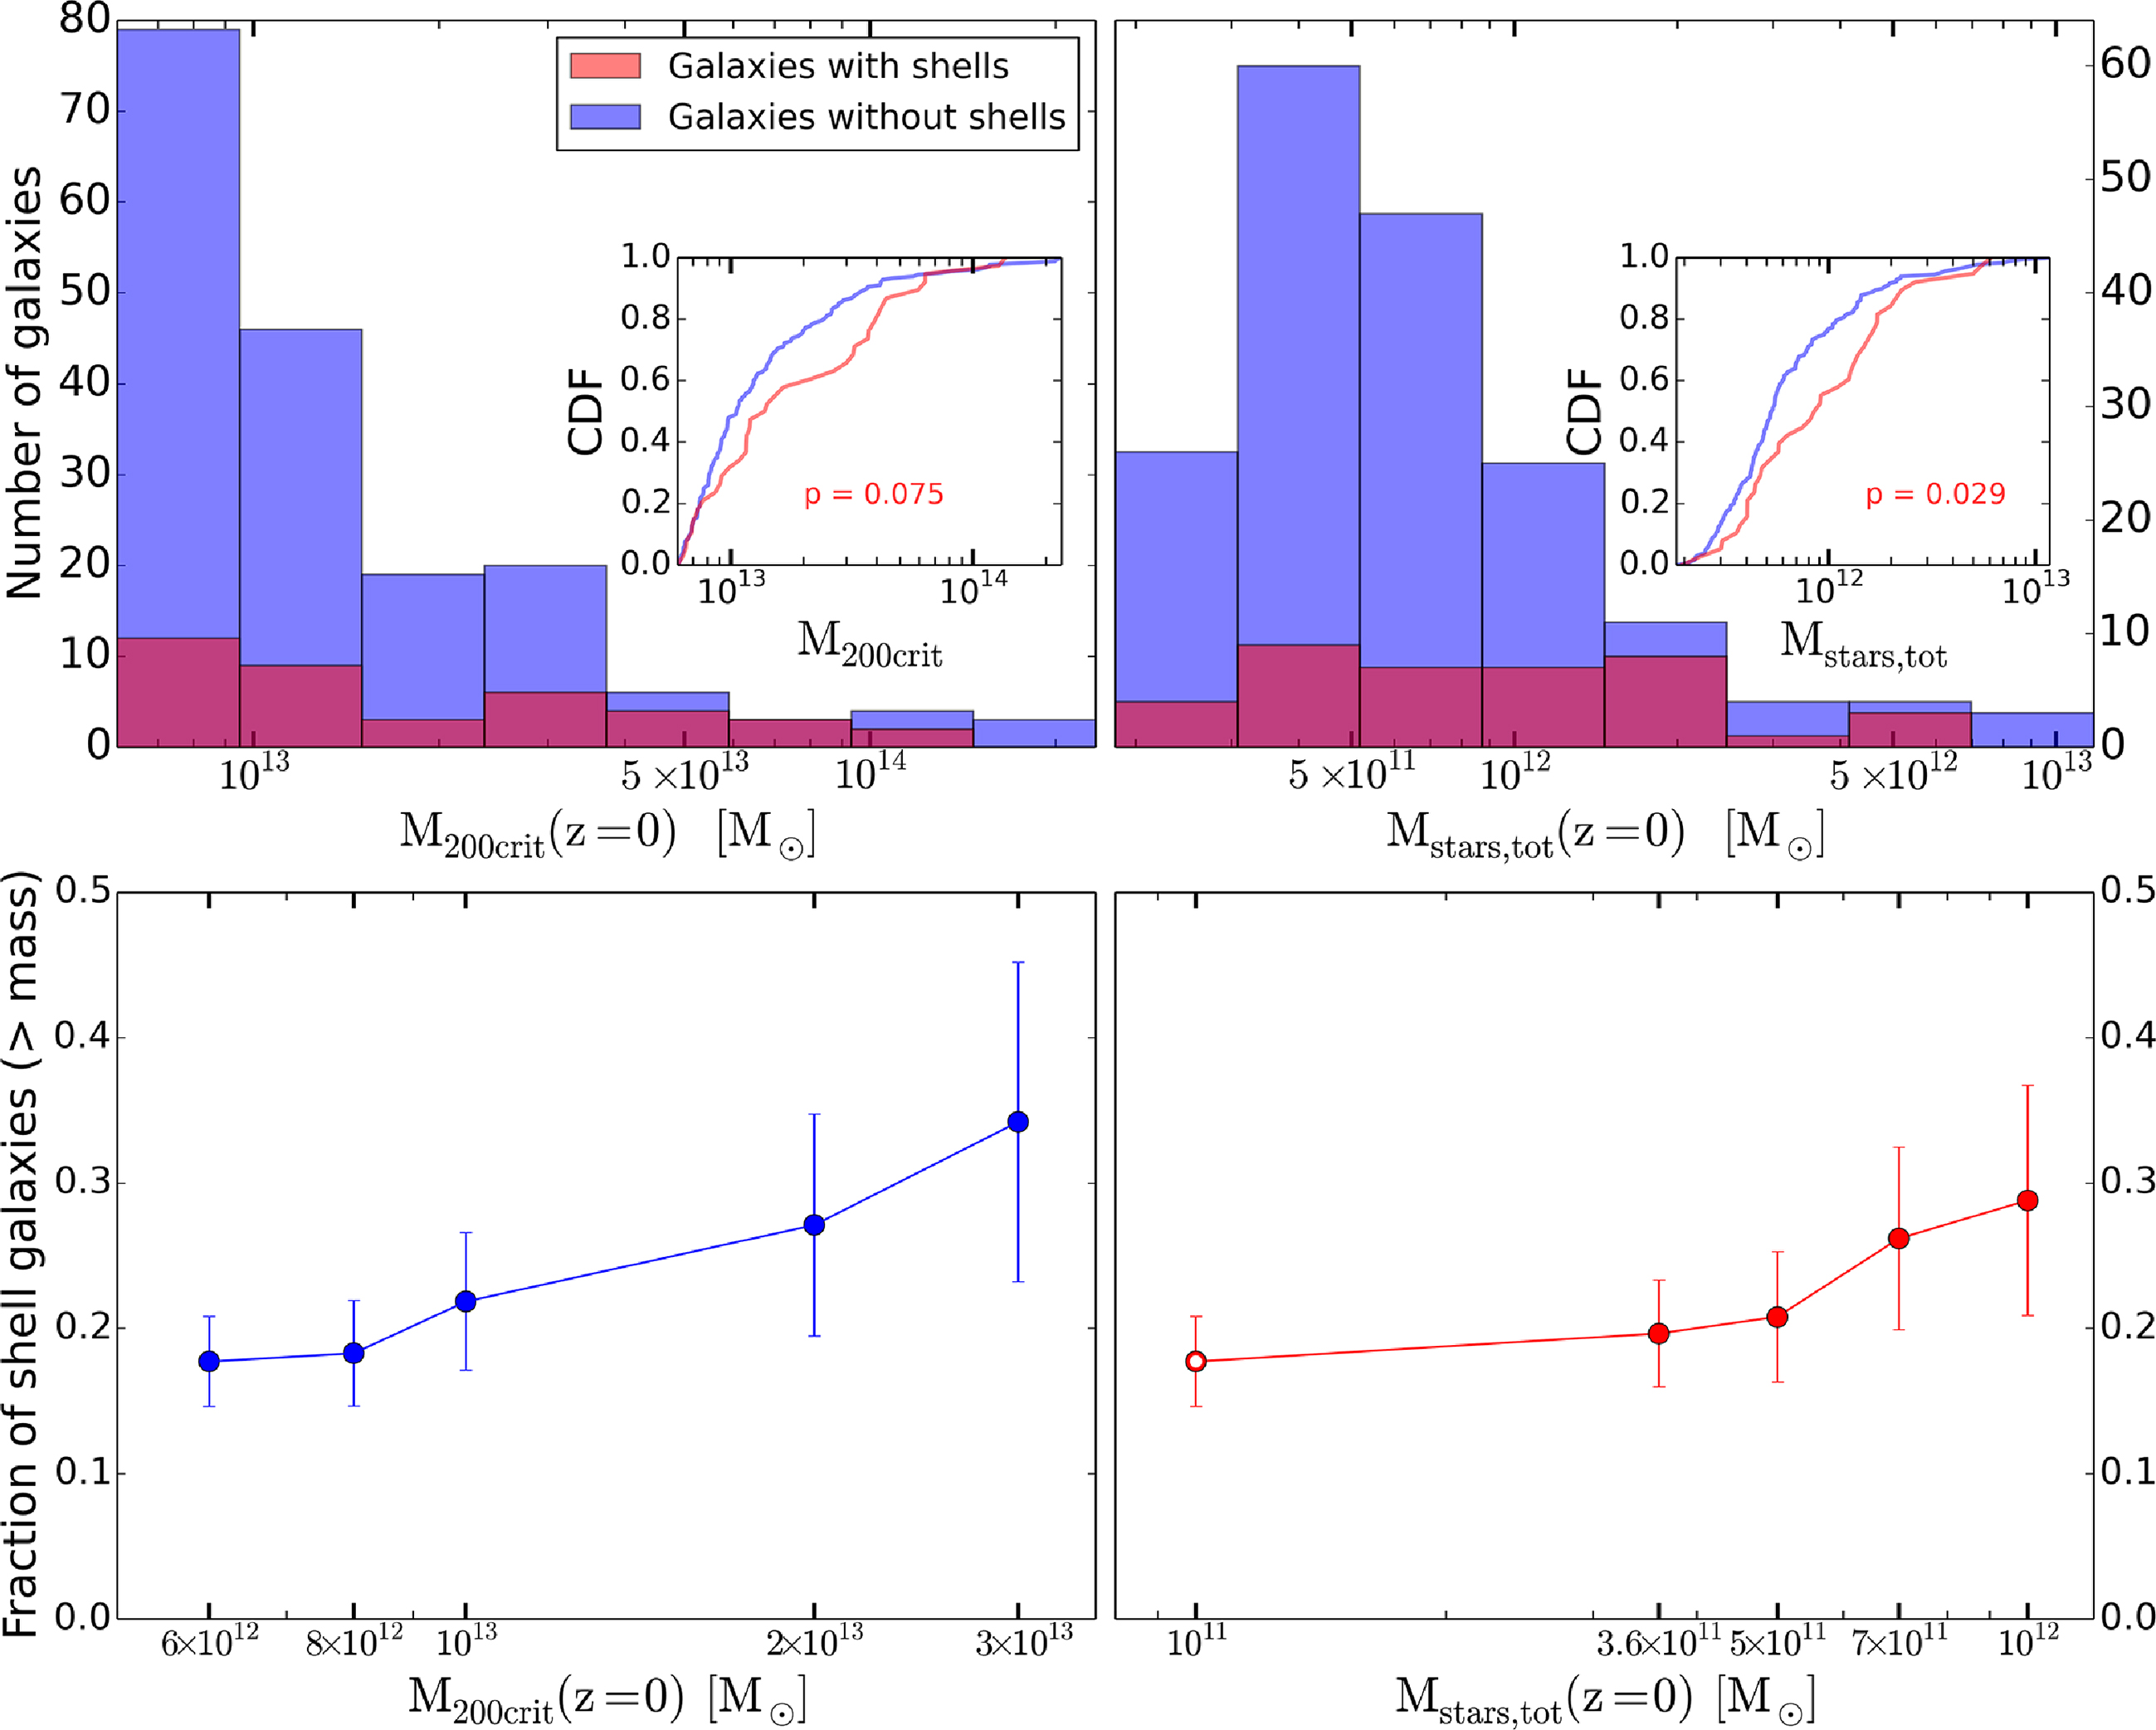
\includegraphics[trim={0 0 0 0}, clip, width=0.8\textwidth]{shellmass.jpeg}			
\caption{Comparación de la distribución de masas de las galaxias con shells y sin shells de la muestra del estudio, tanto para la masa virial \(M_{200\text{crit}}\) (definida como la masa encerrada en el radio del virial de la galaxia\cref{virial}) como para \(M_{stars}\). Fila superior: número de galaxias en cada intervalo de masas con su frecuencia acumulada, donde es evidente que la distribución de las galaxias con shells es más plana. El valor \(p\) resulta de un test de Kolmogorov-Smirnov y representa la (baja) probabilidad de que ambos tipos de galaxias tengan la misma distribución de masa. Cabe destacar que en el último intervalo no se distinguen shells. Fila inferior: se representa la fracción de galaxias con shells sobre el total para cada intervalo de masa, y se observa claramente cómo esta proporción sube para las galaxias de mayor masa. Imagen de \autocite{popFormationIncidenceShell2018} (figura 6). \label{shellmass}}
\end{figure}
\noindent

Hemos establecido que las shells están formadas por las estrellas \textit{ex situ} y, por lo tanto, surgen como consecuencia de los sucesos de fusión entre varias galaxias. La siguiente pregunta es qué condiciones favorecen la aparición de shells frente a los otros tipos de estructuras que mencionamos en la sección \ref{estructuras} \nota{dejar esta referencia solo si cambio las secciones}. \par

El parámetro más importante, tradicionalmente, es la radialidad de la órbita \nota{traducción?} \(v_{r}/|v|\). Cuando \(v_{r}/|v| \approx -1\), la galaxia satélite se acerca a la principal con una trayectoria prácticamente recta y directa a su centro. Al coincidir en el espacio ambas galaxias, la principal extrae una parte de las estrellas de la satélite, de manera que con cada paso de la órbita se forman \enquote{capas} con concentraciones relativamente altas de estrellas, todas distribuidas a lo largo del eje de la órbita \nota{entiendo que suele coincidir con el eje mayor de la galaxia porque el eje mayor queda definido durante la colisión}. Estas capas son las shells. Si la órbita inicial tiene un mayor momento angular, entonces es de esperar que la extracción se lleve a cabo a lo largo de una trayectoria más extendida, y que por lo tanto se formen, en su lugar, corrientes de marea.\par

Sin embargo, en este estudio se observa una vía alternativa para la formación de shells. Cuando ambas galaxias tienen masas del mismo orden de magnitud, de manera que \(\mu = M_{sat}/M_{host} \gtrsim 1:10\), las condiciones para la órbita se relajan y es posible formar shells con trayectorias de colisión más tangenciales, de hasta \(v_{r}/|v| \lesssim -0,5\). Estas grandes fusiones también tendrán más facilidad para producir shells de tipo II. \par

La otra gran variable que determina la capacidad para formar shells y que se puedan observar en \(z=0\) es el tiempo de acreción \(t_{acc}\). Si es demasiado corto (inferior a \(\sim 4\) Gyr), no ha habido suficiente tiempo para que las estrellas puedan extraerse, y aún no habrán podido formar shells. Si es demasiado largo (\(\gtrsim 8\) Gyr), las shells pudieron formarse, pero ya se han mezclado con el entorno desde entonces. En la figura \ref{tri} vemos el \enquote{triángulo} en el que la formación de shells está favorecida, teniendo en cuenta estos tres factores. También se ha de considerar, como dijimos al principio de esta sección \nota{revisar si se cambian las secciones}, la temperatura \nota{relacionar con el principio}

\begin{figure}[h]
\centering
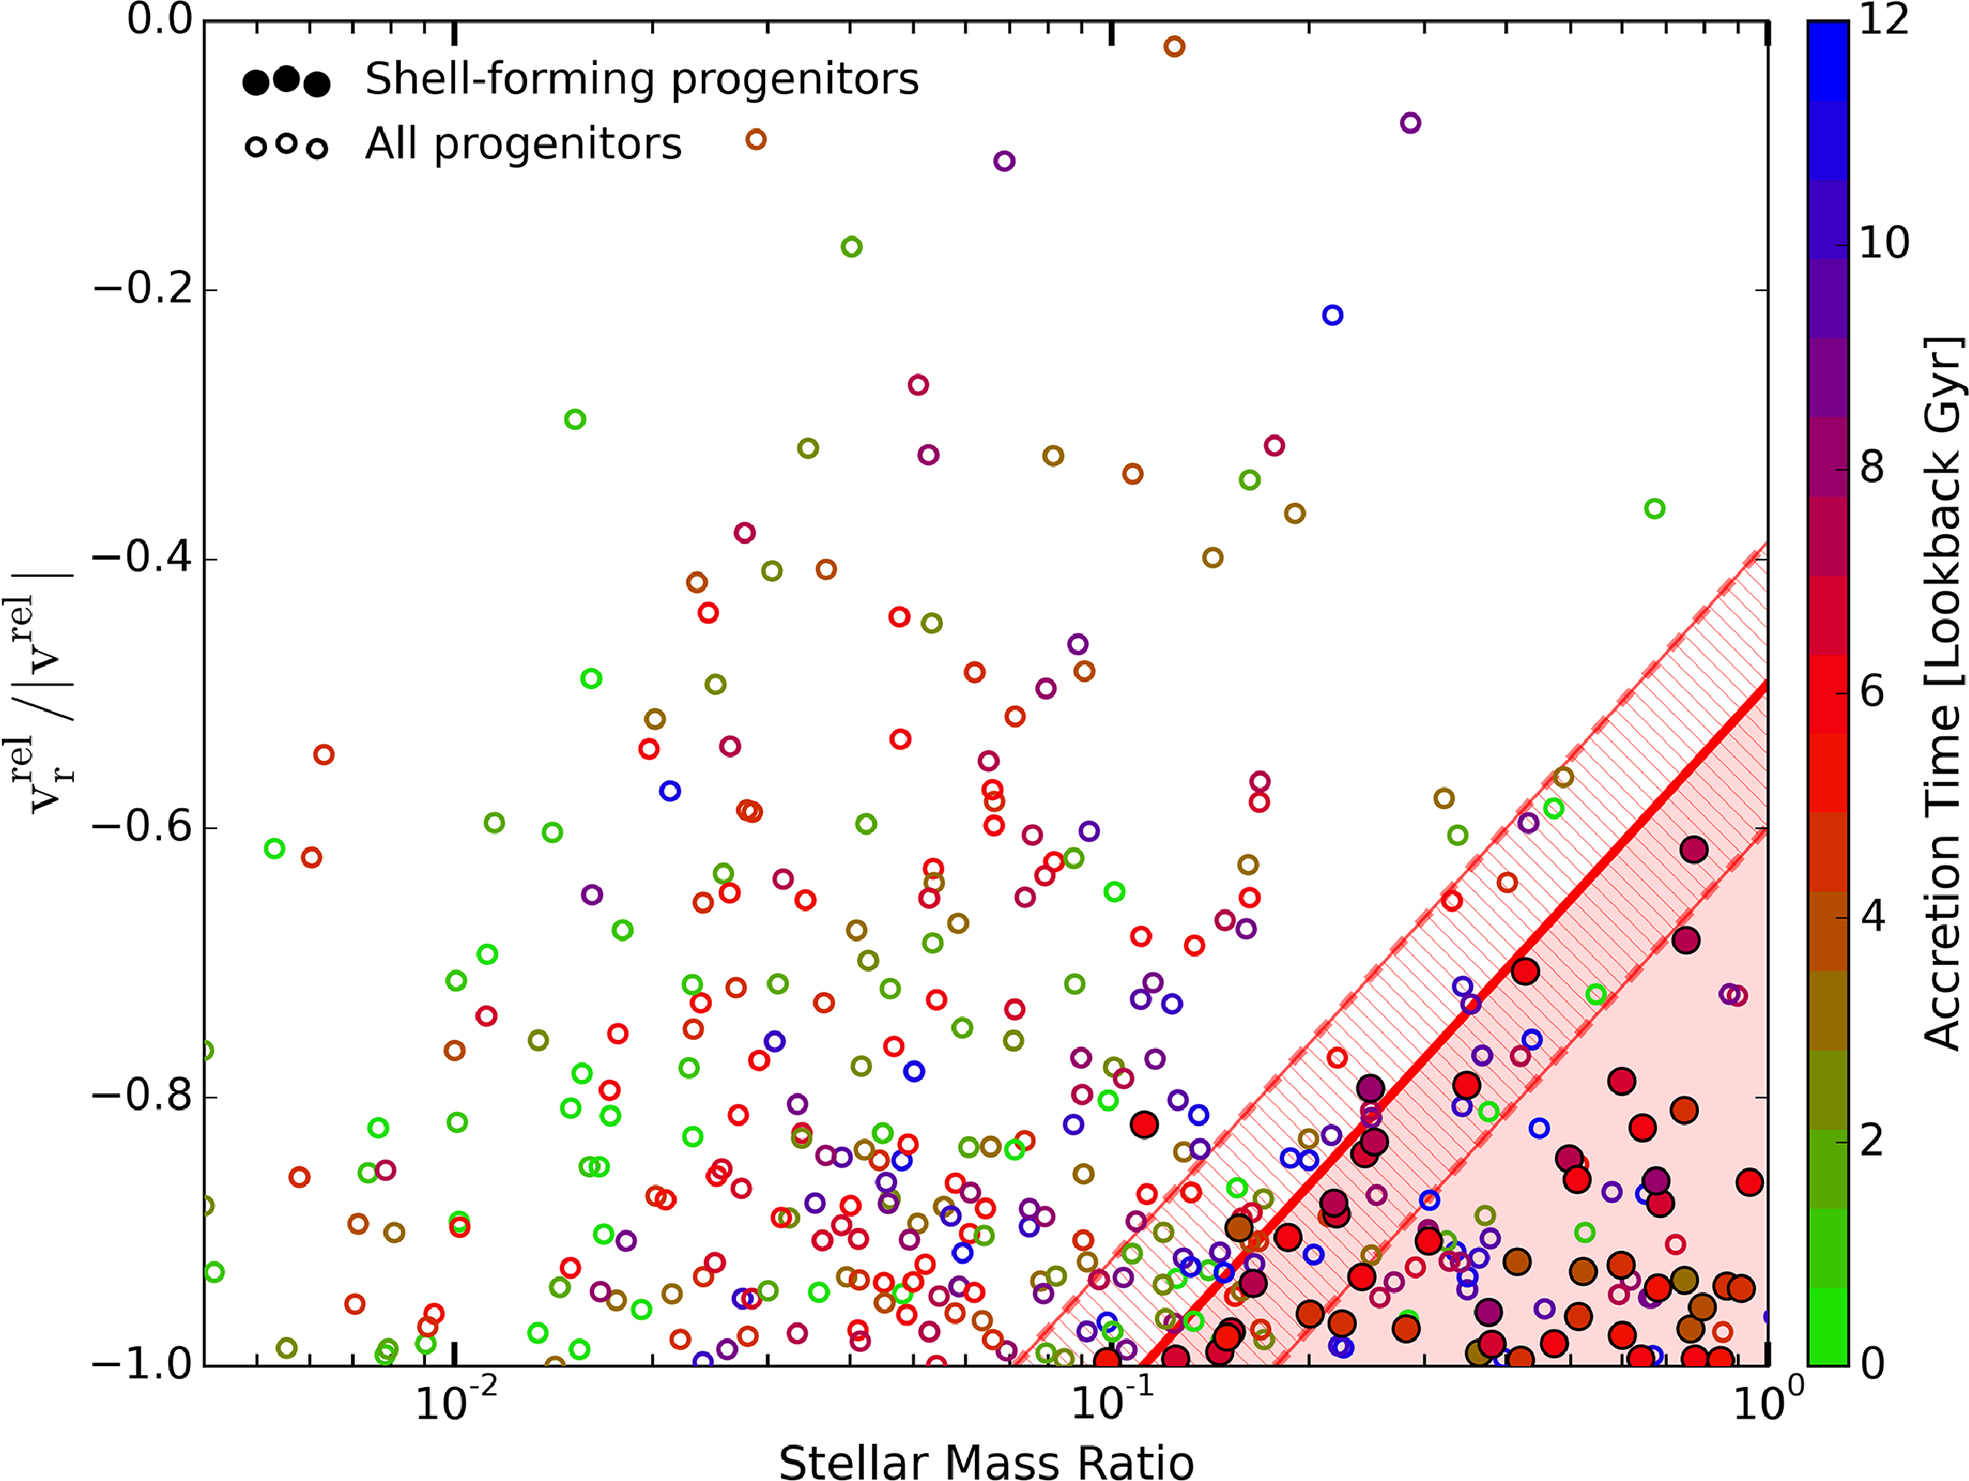
\includegraphics[trim={0 0 0 0}, clip, width=0.7\textwidth]{triangulo.jpeg}			
\caption{Comparación entre las galaxias satélite que forman shells y las que no en el espacio de parámetros \((\mu_{stars}, \, v_{r}/|v|, \, t_{acc})\). Podemos observar que la práctica totalidad de la formación de shells se da en el \enquote{triángulo virtuoso} que combina una \(\mu_{stars}\) alta y una trayectoria relativamente radial, siempre y cuando el \(t_{acc}\) sea el adecuado. Imagen de \autocite{popFormationIncidenceShell2018} (figura 9). \label{tri}}
\end{figure}
\noindent



\begin{figure}[h]
\centering
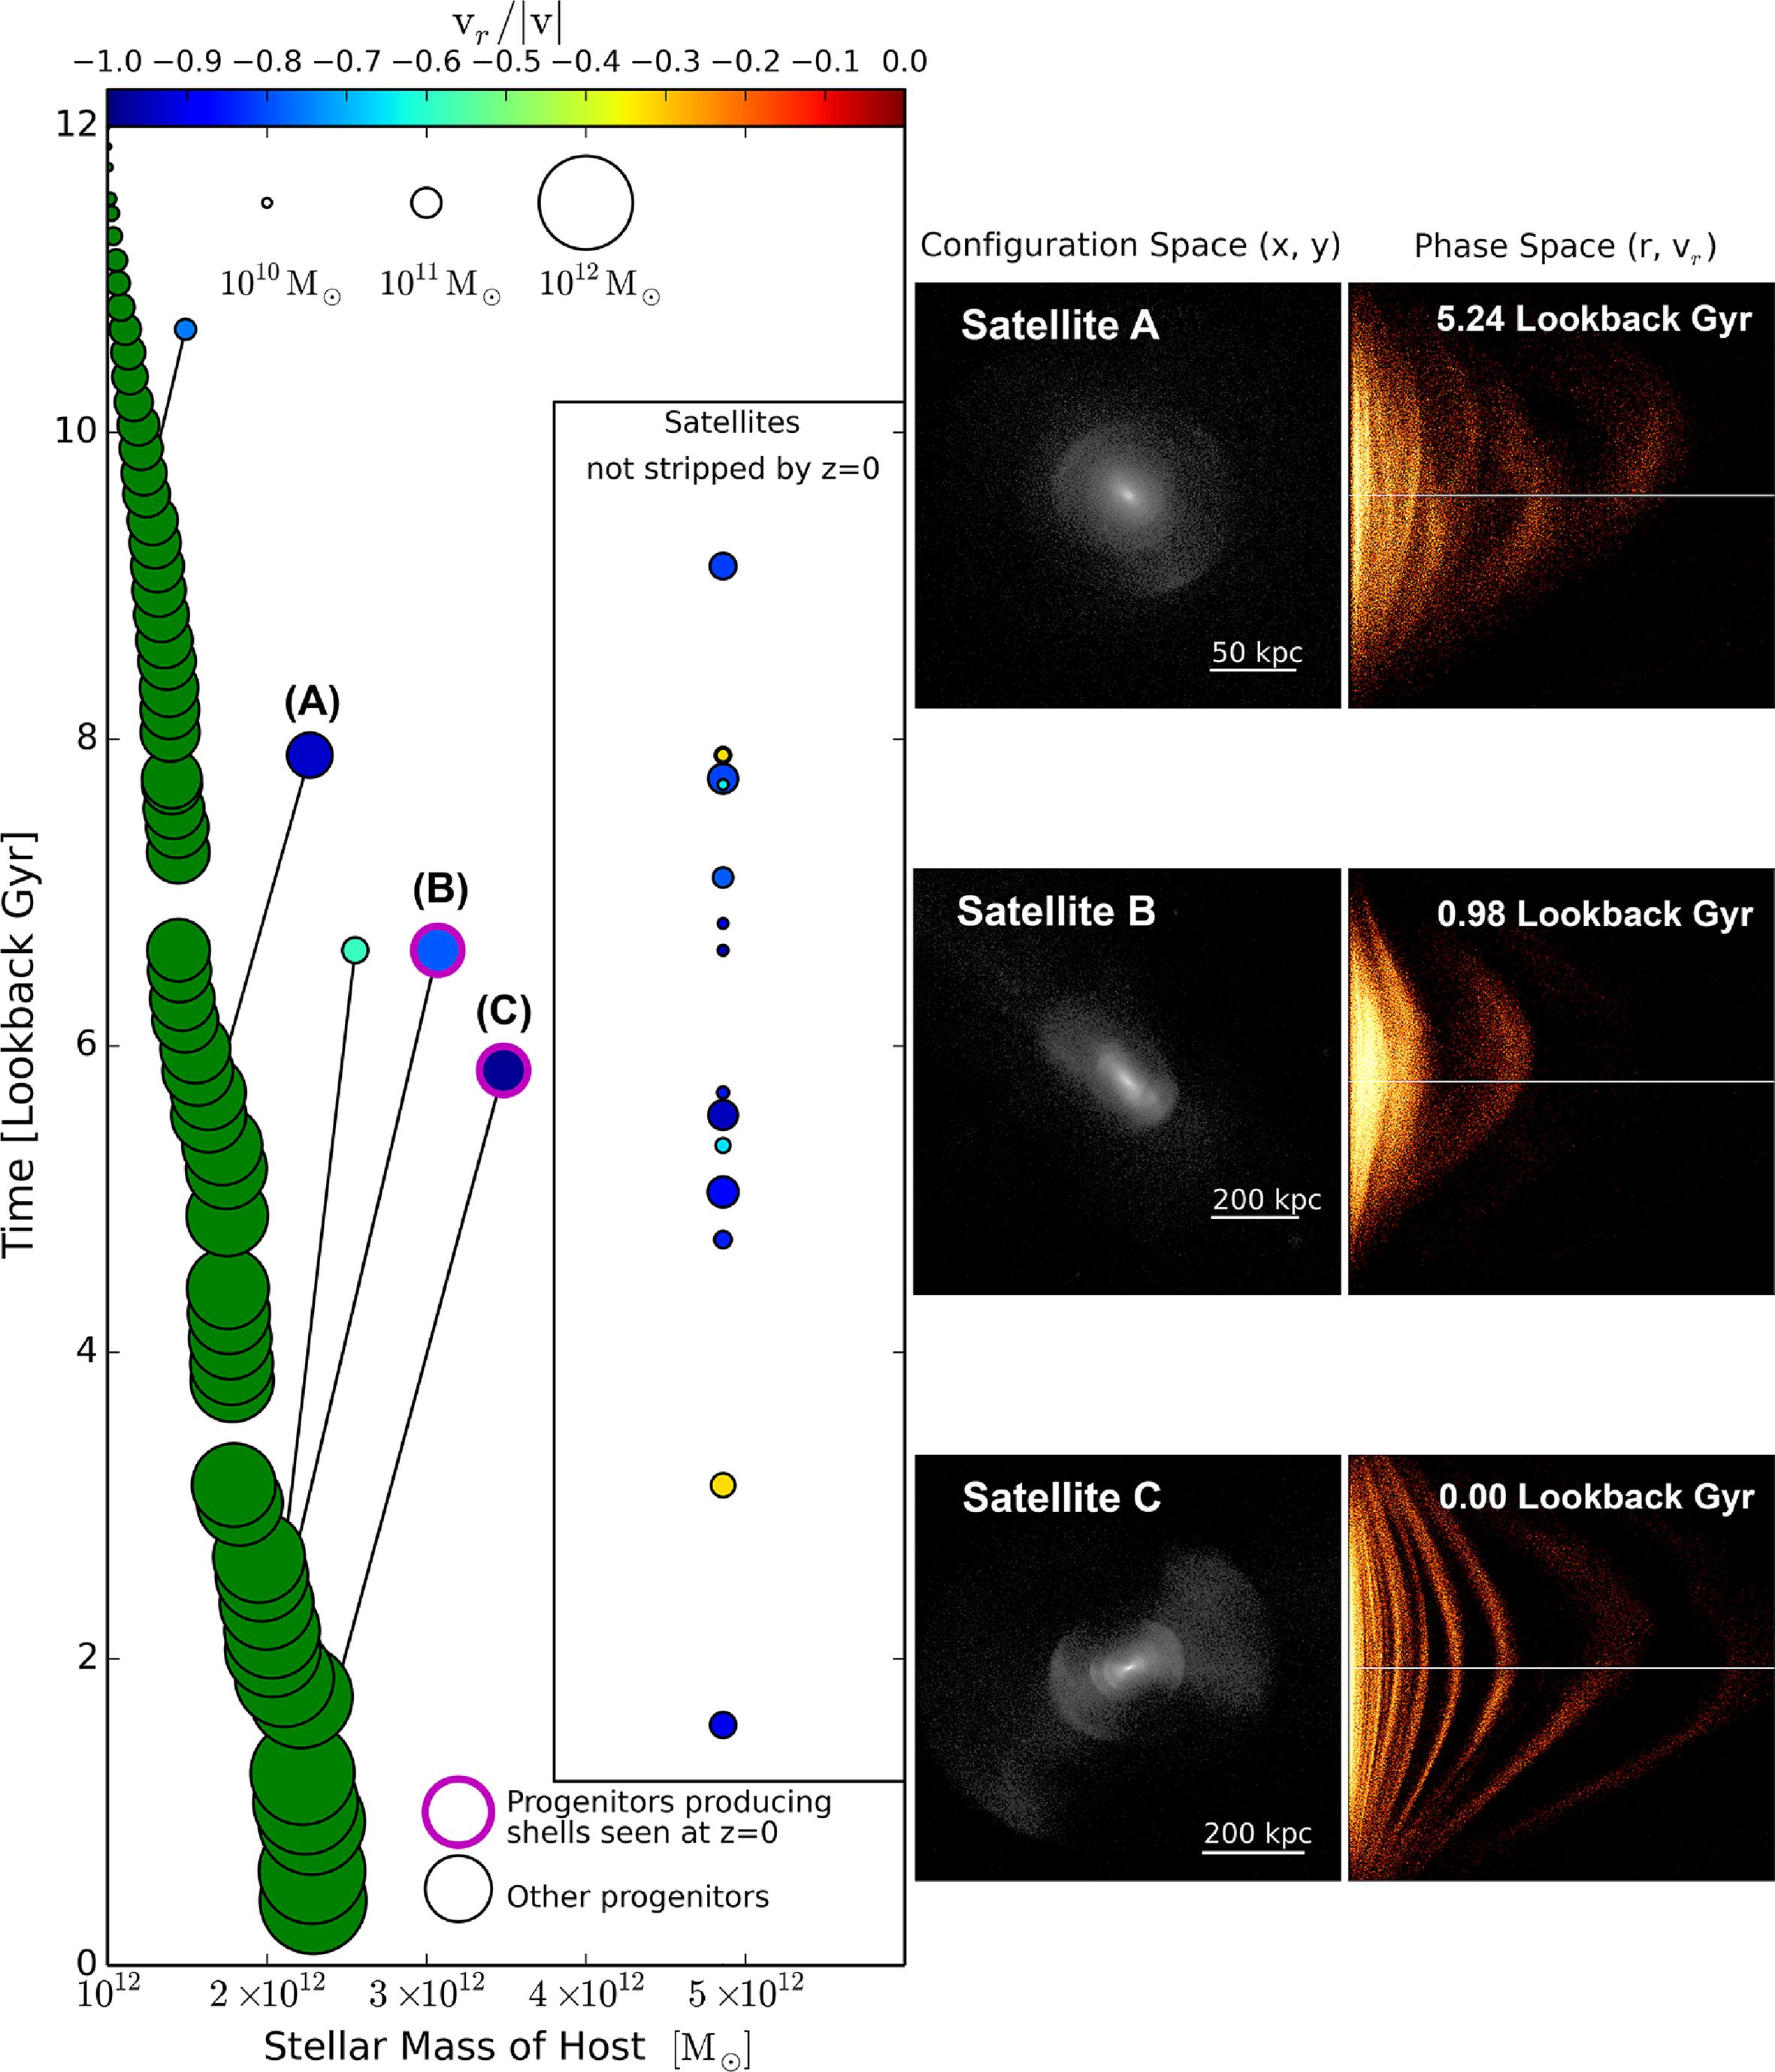
\includegraphics[trim={0 0 0 0}, clip, width=0.7\textwidth]{evoluciongalaxia.jpeg}			
\caption{\nota{escribir pie de figura} Imagen de \autocite{popFormationIncidenceShell2018} (figura 10). \label{evo}}
\end{figure}
\noindent

